\documentclass[10pt, a4paper]{report}
% !TeX program = xelatex
%==================PREAMBOLO=======================%
%%%%%%%%%%%%%%%%%%%%%%%%%%%%%%%%%%%%%%%%%%%%%%%%%%%%%%%%%%%%%%%%%%%%%%%%%%%%%
%% PREAMBLE
%% Reorganized for readability: packages, colors, custom commands, code
%% listing styles, tcolorbox theorem-like environments and title formatting
%% are grouped by purpose. No functional change was made to the original
%% document: only the order of declarations and the comments were edited.
%%%%%%%%%%%%%%%%%%%%%%%%%%%%%%%%%%%%%%%%%%%%%%%%%%%%%%%%%%%%%%%%%%%%%%%%%%%%%


%%%%%%%%%%%%%%%%%%%%%%%%%%%%%%%%%%%%%%%%%%%%%%%%%%%%%%%%%%%%%%%%%%%%%%%%%%%%%
%% 1. PACKAGES
%%%%%%%%%%%%%%%%%%%%%%%%%%%%%%%%%%%%%%%%%%%%%%%%%%%%%%%%%%%%%%%%%%%%%%%%%%%%%

% --- Encoding, language and fonts ---------------------------------------
\usepackage[utf8]{inputenc}
\usepackage[T1]{fontenc}
\usepackage[english]{babel}
\usepackage{mathpazo}          % Palatino font, replaces lmodern to match the image's serif style
\usepackage[scaled]{helvet}    % Helvetica, used for section/subsection titles

% --- Page layout and headers/footers ------------------------------------
\usepackage[paper=a4paper,left=25mm,right=25mm,bottom=25mm,top=25mm]{geometry}
\usepackage{fancyhdr}
\usepackage[Rejne]{fncychap}
\usepackage{titlesec}
\usepackage{titletoc}
\usepackage{needspace}

% --- Math ----------------------------------------------------------------
\usepackage{amsmath}
\usepackage{amssymb}
\usepackage{amsfonts}
\usepackage{mathtools}
\usepackage{mathrsfs}
\usepackage{stmaryrd}
\usepackage{nicefrac, xfrac}

% --- Graphics and TikZ -----------------------------------------------------
\usepackage{graphicx}          % Required for inserting images
\usepackage[export]{adjustbox}
\usepackage{pdfpages}
\usepackage{tikz}
\usepackage{tikz-3dplot}
\usepackage{tikz-cd}
\usepackage{pgfplots}
\usepackage{pgf-pie}
\usetikzlibrary{positioning}

% --- Colors and colored boxes ---------------------------------------------
\usepackage[table,xcdraw]{xcolor}
\usepackage[most]{tcolorbox}
\tcbuselibrary{theorems}

% --- Lists, layout helpers and decorations --------------------------------
\usepackage[shortlabels]{enumitem}
\usepackage{wrapfig}
\usepackage{multicol}
\usepackage{moresize}
\usepackage{fourier-orns}       % Decorative ornaments (used by \flowerLine, \eqImportante)
\usepackage{psvectorian}        % Decorative vectorial ornaments
\usepackage{lipsum}             % Placeholder ("dummy") text
\usepackage{blindtext}          % Placeholder ("dummy") text

% --- Code listings ---------------------------------------------------------
\usepackage{listings}
\usepackage{minted}

% --- Miscellaneous ---------------------------------------------------------
\usepackage{hyperref}


%%%%%%%%%%%%%%%%%%%%%%%%%%%%%%%%%%%%%%%%%%%%%%%%%%%%%%%%%%%%%%%%%%%%%%%%%%%%%
%% 2. COLOR DEFINITIONS
%%%%%%%%%%%%%%%%%%%%%%%%%%%%%%%%%%%%%%%%%%%%%%%%%%%%%%%%%%%%%%%%%%%%%%%%%%%%%

% --- General purpose colors ---
\definecolor{light-gray}{gray}{0.95}
\definecolor{darkgreen}{HTML}{008000}
\definecolor{g}{RGB}{60, 50, 50}

% --- "Sapienza" theme colors ---
\definecolor{sapienza}{HTML}{660f1d}
\definecolor{lightSapienza}{HTML}{e3d3d5}

% --- Cover / decorative colors ---
\definecolor{cop}{HTML}{f7ecd7}
\definecolor{copAut}{HTML}{ababab}
\definecolor{copAut2}{HTML}{c3c3e6}
\definecolor{purcop}{HTML}{d0d3db}
\definecolor{cartaRiciclata}{HTML}{fcfcf7}

% --- Colors used for C / C++ code listings ---
\definecolor{mGreen}{rgb}{0,0.6,0}
\definecolor{mGray}{rgb}{0.5,0.5,0.5}
\definecolor{mPurple}{rgb}{0.58,0,0.82}
\definecolor{backgroundColour}{rgb}{0.95,0.95,0.92}


%%%%%%%%%%%%%%%%%%%%%%%%%%%%%%%%%%%%%%%%%%%%%%%%%%%%%%%%%%%%%%%%%%%%%%%%%%%%%
%% 3. CUSTOM COMMANDS
%%%%%%%%%%%%%%%%%%%%%%%%%%%%%%%%%%%%%%%%%%%%%%%%%%%%%%%%%%%%%%%%%%%%%%%%%%%%%

% --- Colored text shortcuts ------------------------------------------------
\newcommand{\redText}[1]{\color{red}#1\color{black}}
\newcommand{\blueText}[1]{\color{blue}#1\color{black}}
\newcommand{\greenText}[1]{\color{darkgreen}#1\color{black}}
\newcommand{\sapText}[1]{\color{sapienza}#1\color{black}}
\newcommand{\textg}[1]{\color{g}{\textbf{#1}}\color{black}}

% --- Inline code / shell snippets -------------------------------------------
\newcommand{\code}[1]{\colorbox{light-gray}{\texttt{#1}}}
\newcommand{\codee}[1]{\colorbox{white}{\texttt{#1}}}
\newcommand{\shell}[1]{\colorbox{black}{\textcolor{white}{\texttt{#1}}}}
\newcommand{\boxedMath}[1]{\begin{tabular}{|c|}\hline \texttt{#1} \\ \hline\end{tabular} :}

% --- Highlighted paragraph boxes --------------------------------------------
\newcommand\greybox[1]{%
  \vskip\baselineskip%
  \par\noindent\colorbox{light-gray}{%
    \begin{minipage}{\textwidth}#1\end{minipage}%
  }%
  \vskip\baselineskip%
}
\newcommand\sapbox[1]{%
  \vskip\baselineskip%
  \par\noindent\colorbox{lightSapienza}{%
    \begin{minipage}{\textwidth}#1\end{minipage}%
  }%
  \vskip\baselineskip%
}

% --- Statement labels (theorem/definition/etc. headers as plain text) ------
\newcommand{\teo}[1]{{\large\color{sapienza}\textbf{Teorema #1 :\hphantom{a}}}}
\newcommand{\defi}[1]{{\large\color{sapienza}\textbf{Definizione #1 :\hphantom{a}}}}
\newcommand{\prop}[1]{{\color{sapienza}\textbf{Proposizione #1 :\hphantom{a}}}}
\newcommand{\lemma}[1]{{\color{sapienza}\textbf{Lemma #1 :\hphantom{a}}}}
\newcommand{\claim}[1]{{\color{sapienza}\textbf{Claim #1 :\hphantom{a}}}}
\newcommand{\dimo}[1]{{\color{sapienza}\textbf{Dimostrazione #1 :\hphantom{a}}}}
\newcommand{\acc}{\\\hphantom{}\\}
\newcommand{\esempio}[1]{{\acc\large\color{sapienza}\textbf{Esempio #1 \hphantom{a}}\acc}}

% --- Number sets and blackboard-bold symbols --------------------------------
\newcommand{\N}{{\mathbb N}}
\newcommand{\Z}{{\mathbb Z}}
\newcommand{\R}{{\mathbb R}}
\newcommand{\C}{{\mathbb C}}
\newcommand{\K}{{\mathbb K}}
\newcommand{\quat}{{\mathbb H}}
\newcommand{\Prob}{{\mathbb P}}
\newcommand{\VA}{{\mathbb E}}

% --- Calligraphic / script symbols ------------------------------------------
\newcommand{\Sn}{{\mathcal S_n}}
\newcommand{\An}{{\mathcal A_n}}
\newcommand{\E}{{\mathcal E}}
\newcommand{\B}{{\mathcal B}}

% --- Bold vector/greek symbols ----------------------------------------------
\newcommand{\btheta}{{\boldsymbol{\theta}}}
\newcommand{\btau}{{\boldsymbol{\tau}}}
\newcommand{\bomega}{{\boldsymbol{\omega}}}
\newcommand{\Bomega}{{\boldsymbol{\Omega}}}
\newcommand{\bmu}{{\boldsymbol{\mu}}}
\newcommand{\brho}{{\boldsymbol{\rho}}}
\newcommand{\bnu}{{\boldsymbol{\nu}}}
\newcommand{\bsigma}{{\boldsymbol{\sigma}}}
\newcommand{\blambda}{{\boldsymbol{\lambda}}}

% --- Dotted mechanics symbols (velocity/acceleration notation) -------------
\newcommand{\dq}{{\dot{\mathbf q}}}
\newcommand{\de}{{\dot{\mathbf e}}}
\newcommand{\dy}{{\dot{\mathbf y}}}
\newcommand{\ddq}{{\ddot{\mathbf q}}}
\newcommand{\ddy}{{\ddot{\mathbf y}}}
\newcommand{\ve}{{\bar v}}

% --- Group theory / algebra operators ---------------------------------------
\newcommand{\aut}{{\text{Aut}}}
\newcommand{\Span}{{\text{Span}}}
\newcommand{\End}{{\text{End}}}
\newcommand{\cen}{{\text{Centro}}}
\newcommand{\norm}{{\unlhd}}
\newcommand{\ciclS}{{\left \langle }}
\newcommand{\ciclE}{{\right \rangle }}
\newcommand{\bra}[1]{\langle #1 \rangle}
\newcommand{\mcm}{{\text{mcm}}}
\newcommand{\MCD}{{\text{MCD}}}
\newcommand{\rg}{{\text{rg}}}
\newcommand{\supp}{{\text{Supp}}}

% --- Complexity theory symbols -----------------------------------------------
\newcommand{\ridFunc}{{f:\Sigma^*\rightarrow \Sigma^*}}
\newcommand{\rid}{{\le_m^P}}
\newcommand{\blank}{{\sqcup}}

% --- Miscellaneous math symbols and utilities -------------------------------
\newcommand{\quadBrack}[1]{ \llbracket #1 \rrbracket }
\newcommand{\notimplies}{%
  \mathrel{{\ooalign{\hidewidth$\not\phantom{=}$\hidewidth\cr$\implies$}}}}
\newcommand{\tc}{{\text{ tale che }}}
\newcommand{\spaz}{{\text{\hphantom{aa}}}}

% --- Decorative separators ---------------------------------------------------
\newcommand{\flowerLine}{ \begin{center}\decofourleft\hphantom{ }\decoone\hphantom{ }\decofourright\hphantom{}\hphantom{aa}
\decofourleft\hphantom{ }\decoone\hphantom{ }\decofourright\hphantom{}\hphantom{aa}
\decofourleft\hphantom{ }\decoone\hphantom{ }\decofourright\hphantom{}\hphantom{aa}
\decofourleft\hphantom{ }\decoone\hphantom{ }\decofourright\hphantom{}\hphantom{aa} 
\decofourleft\hphantom{ }\decoone\hphantom{ }\decofourright\hphantom{}\hphantom{aa}
\decofourleft\hphantom{ }\decoone\hphantom{ }\decofourright\hphantom{}\hphantom{aa}
\decofourleft\hphantom{ }\decoone\hphantom{ }\decofourright\hphantom{}\hphantom{aa}
\decofourleft\hphantom{ }\decoone\hphantom{ }\decofourright\hphantom{}\hphantom{aa}
\decofourleft\hphantom{ }\decoone\hphantom{ }\decofourright\hphantom{}\hphantom{aa}
\end{center}}
\newcommand{\eqImportante}[1]{\begin{center}\huge\lefthand\hphantom{a}
    \normalsize\texttt{#1}
    \hphantom{aaa}\huge\righthand\end{center}}


%%%%%%%%%%%%%%%%%%%%%%%%%%%%%%%%%%%%%%%%%%%%%%%%%%%%%%%%%%%%%%%%%%%%%%%%%%%%%
%% 4. PAGE STYLE (HEADER / FOOTER)
%%%%%%%%%%%%%%%%%%%%%%%%%%%%%%%%%%%%%%%%%%%%%%%%%%%%%%%%%%%%%%%%%%%%%%%%%%%%%
\fancyhf{}
\pagestyle{fancy}
\renewcommand{\headrulewidth}{0.4pt}


%%%%%%%%%%%%%%%%%%%%%%%%%%%%%%%%%%%%%%%%%%%%%%%%%%%%%%%%%%%%%%%%%%%%%%%%%%%%%
%% 5. CODE LISTING STYLES (C / C++)
%%%%%%%%%%%%%%%%%%%%%%%%%%%%%%%%%%%%%%%%%%%%%%%%%%%%%%%%%%%%%%%%%%%%%%%%%%%%%
% The following styles configure the `listings` package for displaying
% C and C++ source code with syntax highlighting.

\lstdefinestyle{CStyle}{
    backgroundcolor=\color{backgroundColour},   
    commentstyle=\color{mGreen},
    keywordstyle=\color{magenta},
    numberstyle=\tiny\color{mGray},
    stringstyle=\color{mPurple},
    basicstyle=\footnotesize,
    breakatwhitespace=false,         
    breaklines=true,                 
    captionpos=b,                    
    keepspaces=true,                 
    numbers=left,                    
    numbersep=5pt,                  
    showspaces=false,                
    showstringspaces=false,
    showtabs=false,                  
    tabsize=2,
    language=C
}

\lstdefinestyle{CppStyle}{
    backgroundcolor=\color{backgroundColour},   
    commentstyle=\color{mGreen}\ttfamily,
    morecomment=[l][\color{magenta}]{\#}
    keywordstyle=\color{blue}\ttfamily,
    numberstyle=\tiny\color{mGray},
    stringstyle=\color{red}\ttfamily,
    basicstyle=\ttfamily,
    breakatwhitespace=false,         
    breaklines=true,                 
    captionpos=b,                    
    keepspaces=true,                 
    numbers=left,                    
    numbersep=5pt,                  
    showspaces=false,                
    showstringspaces=false,
    showtabs=false,                  
    tabsize=2,
    language=C
}

% Global default `listings` configuration (applied when no style is selected)
\lstset{language=C++,
                basicstyle=\ttfamily,
                keywordstyle=\color{blue}\ttfamily,
                stringstyle=\color{red}\ttfamily,
                commentstyle=\color{green}\ttfamily,
                morecomment=[l][\color{magenta}]{\#}
}


%%%%%%%%%%%%%%%%%%%%%%%%%%%%%%%%%%%%%%%%%%%%%%%%%%%%%%%%%%%%%%%%%%%%%%%%%%%%%
%% 6. TCOLORBOX THEOREM-LIKE ENVIRONMENTS
%%%%%%%%%%%%%%%%%%%%%%%%%%%%%%%%%%%%%%%%%%%%%%%%%%%%%%%%%%%%%%%%%%%%%%%%%%%%%
% Each environment below renders a boxed, numbered statement (definition,
% theorem, proposition, ...) with a "tab" style title in the top-left
% corner, following the same visual template.

\newtcbtheorem[number within=section]{boxdefinition}{Definition}{
    enhanced,
    before skip=15pt, after skip=15pt,
    colback=white,                          % white background for the text
    colframe=sapienza!50!black!30,          % border color (light green/gray)
    fonttitle=\bfseries,
    coltitle=black,
    % Style of the top-left "tab"
    attach boxed title to top left={xshift=10mm, yshift=-3.5mm, yshifttext=-1mm},
    boxed title style={
        colframe=sapienza!50!black!30,
        arc=3mm,
        outer arc=3mm,
        left=10pt, right=10pt,
        top=2pt, bottom=2pt,
        % Green gradient shading, as in the reference image
        interior style={left color=sapienza!20, right color=sapienza!40}
    },
    % Rounding of the main box
    arc=4mm,
    separator sign none,                    % removes the automatic colon so it can be added manually in the title
    description font=\normalfont\bfseries,
    description delimiters={: }{ }          % formats the title as "Definition 2.1: Title"
}{def}

\newtcbtheorem[number within=section]{boxtheorem}{Theorem}{
    enhanced,
    before skip=15pt, after skip=15pt,
    colback=white,
    colframe=sapienza!50!black!30,
    fonttitle=\bfseries,
    coltitle=black,
    attach boxed title to top left={xshift=10mm, yshift=-3.5mm, yshifttext=-1mm},
    boxed title style={
        colframe=sapienza!50!black!30,
        arc=3mm,
        outer arc=3mm,
        left=10pt, right=10pt,
        top=2pt, bottom=2pt,
        interior style={left color=sapienza!20, right color=sapienza!40}
    },
    arc=4mm,
    separator sign none,
    description font=\normalfont\bfseries,
    description delimiters={: }{ }
}{def}

\newtcbtheorem[number within=section]{boxproposition}{Proposition}{
    enhanced,
    before skip=15pt, after skip=15pt,
    colback=white,
    colframe=sapienza!50!black!30,
    fonttitle=\bfseries,
    coltitle=black,
    attach boxed title to top left={xshift=10mm, yshift=-3.5mm, yshifttext=-1mm},
    boxed title style={
        colframe=sapienza!50!black!30,
        arc=3mm,
        outer arc=3mm,
        left=10pt, right=10pt,
        top=2pt, bottom=2pt,
        interior style={left color=sapienza!30, right color=sapienza!50}
    },
    arc=4mm,
    separator sign none,
    description font=\normalfont\bfseries,
    description delimiters={: }{ }
}{def}

\newtcbtheorem[number within=section]{boxequation}{Equation}{
    enhanced,
    before skip=15pt, after skip=15pt,
    colback=white,
    colframe=sapienza!50!black!30,
    fonttitle=\bfseries,
    coltitle=black,
    attach boxed title to top left={xshift=10mm, yshift=-3.5mm, yshifttext=-1mm},
    boxed title style={
        colframe=sapienza!50!black!30,
        arc=3mm,
        outer arc=3mm,
        left=10pt, right=10pt,
        top=2pt, bottom=2pt,
        interior style={left color=sapienza!30, right color=sapienza!50}
    },
    arc=4mm,
    separator sign none,
    description font=\normalfont\bfseries,
    description delimiters={: }{ }
}{def}

\newtcbtheorem[number within=section]{boxlemma}{Lemma}{
    enhanced,
    before skip=15pt, after skip=15pt,
    colback=white,
    colframe=sapienza!50!black!30,
    fonttitle=\bfseries,
    coltitle=black,
    attach boxed title to top left={xshift=10mm, yshift=-3.5mm, yshifttext=-1mm},
    boxed title style={
        colframe=sapienza!50!black!30,
        arc=3mm,
        outer arc=3mm,
        left=10pt, right=10pt,
        top=2pt, bottom=2pt,
        interior style={left color=sapienza!30, right color=sapienza!50}
    },
    arc=4mm,
    separator sign none,
    description font=\normalfont\bfseries,
    description delimiters={: }{ }
}{def}

\newtcbtheorem[number within=section]{boxobservation}{Observation}{
    enhanced,
    before skip=15pt, after skip=15pt,
    colback=white,
    colframe=sapienza!50!black!30,
    fonttitle=\bfseries,
    coltitle=black,
    attach boxed title to top left={xshift=10mm, yshift=-3.5mm, yshifttext=-1mm},
    boxed title style={
        colframe=sapienza!50!black!30,
        arc=3mm,
        outer arc=3mm,
        left=10pt, right=10pt,
        top=2pt, bottom=2pt,
        interior style={left color=sapienza!30, right color=sapienza!50}
    },
    arc=4mm,
    separator sign none,
    description font=\normalfont\bfseries,
    description delimiters={: }{ }
}{def}

\newtcbtheorem[number within=section]{boxpostulate}{Postulate}{
    enhanced,
    before skip=15pt, after skip=15pt,
    colback=white,
    colframe=sapienza!50!black!30,
    fonttitle=\bfseries,
    coltitle=black,
    attach boxed title to top left={xshift=10mm, yshift=-3.5mm, yshifttext=-1mm},
    boxed title style={
        colframe=sapienza!50!black!30,
        arc=3mm,
        outer arc=3mm,
        left=10pt, right=10pt,
        top=2pt, bottom=2pt,
        interior style={left color=sapienza!30, right color=sapienza!50}
    },
    arc=4mm,
    separator sign none,
    description font=\normalfont\bfseries,
    description delimiters={: }{ }
}{def}


%%%%%%%%%%%%%%%%%%%%%%%%%%%%%%%%%%%%%%%%%%%%%%%%%%%%%%%%%%%%%%%%%%%%%%%%%%%%%
%% 7. SECTION / SUBSECTION TITLE FORMATTING
%%%%%%%%%%%%%%%%%%%%%%%%%%%%%%%%%%%%%%%%%%%%%%%%%%%%%%%%%%%%%%%%%%%%%%%%%%%%%

% Section titles: Helvetica, large bold number, colored rule underneath
\titleformat{\section}
  {\needspace{3\baselineskip} % requires at least 3 lines of free space before the title
   \fontfamily{phv}\selectfont\huge\bfseries} 
  {\color{sapienza}\fontsize{20}{20}\selectfont\thesection} 
  {12pt} 
  {} 
  [\vspace{2pt}\nopagebreak\color{sapienza!40}\hrule height 3pt]

% Subsection titles: same style, slightly smaller
\titleformat{\subsection}
  {\needspace{2\baselineskip} % requires at least 2 lines of free space before the title
   \fontfamily{phv}\selectfont\Large\bfseries} 
  {\color{sapienza}\fontsize{16}{16}\selectfont\thesubsection} 
  {12pt} 
  {} 
  [\vspace{2pt}\nopagebreak\color{sapienza!40}\hrule height 1.5pt]
\newcommand{\y}{{\mathbf y}}
\newcommand{\q}{{\mathbf q}}
\usepackage{algorithm}
\usepackage{algpseudocode}
 \usepackage{multirow}
\newcommand{\titolo}{Autonomous And Mobile Robotics}

 %TOGLI COMMENTO SE USI XELATEX
%\usepackage{fontspec}
\title{\titolo} %========TITOLO========%
\author{Marco Casu}
\date{\vspace{-5ex}}
\begin{document}

%==================COPERTINA=======================%
\begin{titlepage}
    \centering
     
    
\includegraphics[width=0.6\textwidth]{../../preamble/Stemma_sapienza.png} 
    \par\vspace{2.5cm}
    
    {\huge \textsc{``Sapienza'' University of Rome}}
    \par\vspace{0.5cm}
    {\Large \textsc{Faculty of Information Engineering,\\ Computer Science and Statistics}} \\[1.5ex]
    {\Large \textsc{Department of Computer, Control\\ and Management Engineering}}
    \\[1.5ex]
    {\Large \textsc{Master's degree in Artificial Intelligence and Robotics
}}
    
    \vspace{2.5cm} % Spazio verticale regolabile
    
    \rule{\textwidth}{2pt} \\
    \vspace{0.5cm}
    {\fontsize{35}{70} \selectfont \textbf{\titolo}} \\
    \vspace{0.35cm}
    \rule{\textwidth}{2pt}
    
    \vspace{0.5cm}
    {\Large Lecture notes}
    
    \vfill % Spinge il contenuto successivo in basso
    
    {\textit{Author}} \\
    {\large{Marco Casu}}
    
    \vspace{2cm}
    
    {\large \today}
    
\end{titlepage}
%===================FINE COPERTINA======================%
\newpage
%\pagecolor{cartaRiciclata}%\setmainfont{Algerian}
\Large
This document summarizes and presents the topics for the \titolo course for the Master's degree in Artificial Intelligence and Robotics at Sapienza University of Rome. The document is free for any use. If the reader notices any typos, they are kindly requested to report them to the author.
\vfill
\begin{figure}[h!]
    \raggedright
    
\includegraphics[width=0.4\textwidth,right ]{../../preamble/tomodachi.pdf} 
\end{figure}
\newpage %\setmainfont{Times New Roman}
\normalsize

\tableofcontents 
\newpage

%==================FOOTER e HEADER=======================%
\fancyhf{}
\fancyhead[L]{\nouppercase{\leftmark}}
\fancyhead[R]{Section \thesection}
\fancyfoot[C]{\thepage}
\fancyfoot[L]{\titolo}
\fancyfoot[R]{Marco Casu}
%\fancyfoot[R]{\setmainfont{Palace Script MT}\huge Marco Casu \setmainfont{Times New Roman}}
%==================FOOTER e HEADER=======================%
%==================INIZIO======================%
\chapter{Wheeled Mobile Robots}
\section{Configuration Space}   
We can define a robot as a collection of $n_b$ bodies moving in an operative space, denoted $W$ and called the \textbf{workspace}. $W$ can be $\R^2$ (if the robot moves on a plane, like a planar 2R) as well as $\R^3$, if the robot moves in the space. For example, an elbow-type spatial manipulator is a system of $n_b=3$ rigid bodies moving in $W=\R^3$. A quadrotor is a single body ($n_b=1$) moving in the same workspace $W=\R^3$. 

To describe the complete pose of a planar 2R manipulator, we might use the position vector and roll-pitch-yaw angles for the two bodies, by requiring a total of 12 parameters for the whole system, despite that, we know that 2 variables are enough to describe the whole configuration of the system.
\begin{boxdefinition}{Configuration}{}
The configuration of a robot is a \textbf{minimum} set of parameters that allows one to specify the posture\footnote{
    with posture, we indicate the position of all the points of the robot.
} of the robot in the workspace.
\end{boxdefinition}
The configuration of a robot can be defined in several ways, and a choice of a set of parameters is not unique, despite that, each robot always has a \textit{minimum number} of parameters. We usually denote $\q$ the configuration vector:\begin{equation}
    \q=\begin{pmatrix}
        q_1\\ \vdots\\ q_n 
    \end{pmatrix}
\end{equation}
in our context, it usually describes the Cartesian coordinates of a single body robot, or the angular coordinates of the body parts. The Cartesian coordinates have values in a Euclidean space, as $\R^2$ or $\R^3$, while the angular coordinates take values in a non-Euclidean space, such as the special orthogonal group $SO(3)$, the group of all the orthogonal $3\times 3$ matrices  with determinant $+1$, this group describes the orientation of a body in a 3D Euclidean space.
\begin{boxdefinition}{Configuration Space}{}
    The configuration space, usually denoted $\mathcal C$, is the set of all possible values of the configuration of a robot. The \textit{dimension} of $\mathcal C$ is the number $n$ of parameters (generalized coordinates) in $\q$.
\end{boxdefinition}
Let's see an example: consider a disk robot that moves on a plane, that can also rotate along its main axis to point towards a desired direction, shown in Figure \ref{disc_tick}.
\begin{figure}[H]
    \centering
    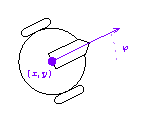
\includegraphics[width=0.2\textwidth ]{images/disc_tick.eps}
    \caption{Disc robot with a tick in $\R^2$.}
    \label{disc_tick}
\end{figure}
Its configuration is given by two Cartesian coordinates $(x,y)$ and a value $\varphi\in SO(2)$ representing the angle between the tick and the horizontal axis. Hence, its configuration space is:\begin{equation}
    \mathcal C = \R^2\times SO(2)=SE(2)
\end{equation}
and it's not Euclidean, despite being called \textit{special Euclidean group}. A polyhedral robot that can freely move in space is described by three Cartesian coordinates $(x,y,z)$ and three roll-pitch-yaw angles $(\alpha,\beta,\gamma)$ describing its orientation, hence the configuration space is $SE(3)$:
\begin{equation}
    \mathcal C = \R^3\times SO(3)=SE(3).
\end{equation}
We have seen in previous courses of robotics that the number of generalized coordinates of an  $n$-link serial manipulator is exactly $n$.
\subsection{Topology of a Space}
We are interested in describing the configuration space of a given manipulator, since it's not Euclidean (in most cases), we would like to have an idea of how to navigate this space. Before defining formally what a \textit{topology} is, we give some examples.\bigskip 

A 2R planar manipulator can be described by two angles, hence two values in $SO(2)$, so its configuration space is\begin{equation}
    \mathcal C = SO(2)\times SO(2)=SO(2)^2
\end{equation}
Let's try to represent graphically $\mathcal C$. We might represent a configuration as a point in the Cartesian plane:
\begin{figure}[H]
    \centering
    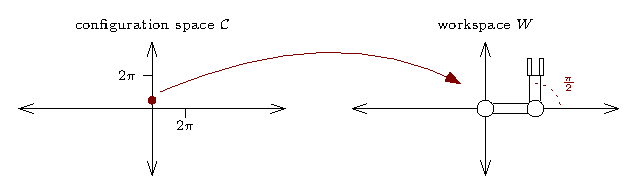
\includegraphics[width=0.8\textwidth ]{images/configuration_2R.eps}
\end{figure}
The problem of this representation is that different configurations $\q\in \mathcal C$ map to the same posture of the robot in $W$, as shown in Figure \ref{not_injective}.
\begin{figure}[H]
    \centering
    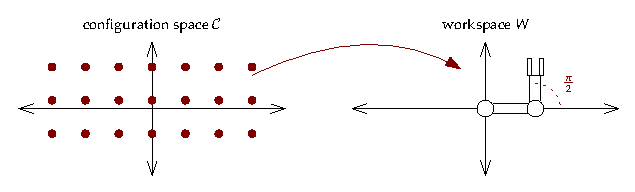
\includegraphics[width=0.8\textwidth ]{images/configuration_2R_notInjective.eps}
    \caption{Different configurations map to the same posture.}
    \label{not_injective}
\end{figure}
To overcome this problem, we might try to represent the configuration space as a square in the plane $[0,2\pi)\times [0,2\pi)$:
\begin{figure}[H]
    \centering
    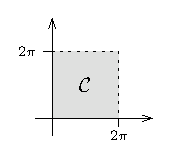
\includegraphics[width=0.3\textwidth ]{images/2pi_times_2pi.eps}
\end{figure}
This representation also presents a problem: The distance between two configurations in $\mathcal C$ does not represent the true distance between two postures in the workspace: Two very distant configurations $\q_a$ and $\q_b$ in $\mathcal C$ can be mapped to two very close postures in $W$:
\begin{figure}[H]
    \centering
    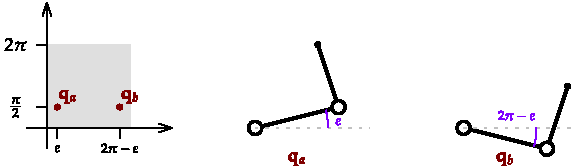
\includegraphics[width=0.9\textwidth ]{images/a_b_distance.pdf}
\end{figure}
This representation is said to be \textbf{not topologically correct}. To give a correct representation of $\mathcal C$ we need to introduce the concept of \textbf{manifold}. We will not give a formal and complete definition (as given in topology or differential geometry courses).
\begin{boxdefinition}{Manifold (loose definition)}{}
    A \textbf{manifold} is a topological space that is locally homeomorphic to $\R^n$.
\end{boxdefinition}
As we should know from previous robotics courses, the configuration space of a 2R is a torus, a manifold that is locally homeomorphic to $\R^2$, and can be visualized in the 3D space through an embedding as shown in Figure \ref{torus}.
\begin{figure}[H]
    \centering
    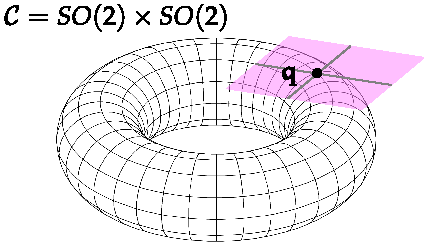
\includegraphics[width=0.4\textwidth ]{images/torus.pdf}
    \caption{3D representation of a torus.}
    \label{torus}
\end{figure}
\subsection{Distance in the Configuration Space}
\begin{boxdefinition}{Distance in the Configuration Space}{distance}
    Given a configuration space $\mathcal C$, the \textbf{distance} is a function $d:\mathcal C\times \mathcal C \to \R$ such that, for each $\q_a,\q_b,\q_c$ in $\mathcal C$ we have:\begin{align}
        &d(\q_a,\q_b)\ge 0\\ 
        &d(\q_a,\q_b)=0\iff \q_a=\q_b\\
        &d(\q_a,\q_b)=d(\q_b,\q_a)\\
        &d(\q_a,\q_b)\le d(\q_a,\q_c)+d(\q_c,\q_b).
    \end{align}
\end{boxdefinition}
\noindent We know how the distance between two vectors $\mathbf u,\mathbf v$ in $\R^n$ is given by $\|\mathbf u - \mathbf v\|$. The distance between two points is the \textit{shortest path} between them, for a general manifold, this path is not always a straight line as for the Euclidean space.
\begin{boxdefinition}{Geodesic}{}
    For a general manifold, the shortest path between two points is called \textbf{geodesic}, and the distance between the points is the length of their geodesic.
\end{boxdefinition}
\noindent For example, consider the shortest path between two points on the surface of a sphere (a 2-manifold): the geodesic lies on the great circle (the circle with the biggest radius that passes through the two points), as shown in Figure \ref{sphere_geodesic}. In general, for an arbitrary manifold, it is hard to determine the geodesic between two points.
\begin{figure}[H]
    \centering
    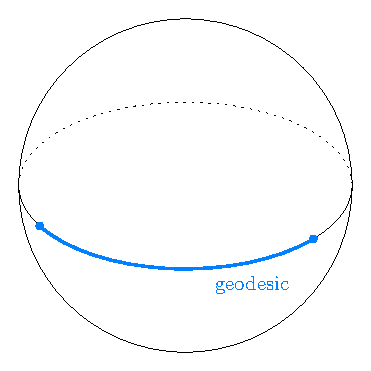
\includegraphics[width=0.25\textwidth ]{images/geodesic_sphere.eps}
    \caption{Geodesic on a sphere.}
    \label{sphere_geodesic}
\end{figure}
In the robotics context, we want to define the distance between two postures of a robot, this distance is defined in the workspace $W$, and to define that we don't need to specify directly the distance between their respective configurations in $\mathcal C$ (it would be harder to find the geodesic on $\mathcal C$).\bigskip 

\noindent Given a robot and its current configuration $\q$, we can define two functions:\begin{itemize}
    \item $B(\q)$ is a function that assigns to $\q$ the volume (exact region) of the workspace that the robot occupies when it is in the configuration $\q$, so it assigns to each configuration  $\q\in\mathcal C$ a set of points in $\R^3$.
    \item $\mathbf p(\q)$ is a function that assigns to $\q$ the exact position of a certain point of the robot when it's in the configuration $\q$.
\end{itemize}
For example, we might let $\mathbf p$ be the center of mass of the manipulator, and observe how it changes by varying $\q\in \mathcal C$. One simple way to define a distance metric is to consider the maximum Euclidean distance between two points of the manipulator in two different configurations:\begin{equation}\label{displacement_metric}
    d(\q_a,\q_b)=\max_{\mathbf p\in \text{robot}}\|\mathbf p(\q_a)-\mathbf p(\q_b)\|
\end{equation}
This distance is called \textbf{displacement metric}. Notice how in the definition we are writing $\mathbf p \in \text{robot}$, by letting robot to be the set of all the points in the structure of the manipulator, which clearly depend on the current configuration. This kind of metric works under the assumption that, if the region occupied by the robot is similar in two different postures, then the distance between their respective configurations is small:\begin{equation}
    B(\q_a)\simeq B(\q_b)\implies d(\q_a,\q_b)\simeq 0.
\end{equation}
\begin{figure}[H]
    \centering
    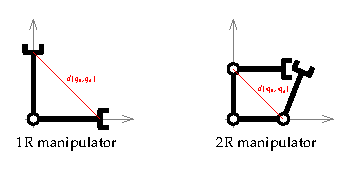
\includegraphics[width=0.6\textwidth ]{images/displacement_metric.eps}
\end{figure}
To compute the distance in Equation \eqref{displacement_metric}, we should check each point of the robot, and in general this is an infinite and uncountable set. If the links are polygonal shapes, the problem becomes finite, since it is possible to find the maximum distance between any pair of polytopes in the three dimensional space. 

A more computationally feasible approach is to check only for a finite set of points in the robot structure, called \textbf{control points}. Let \begin{equation}
    P=\{\mathbf p_1,\mathbf p_2,\dots, \mathbf p_c\}
\end{equation}
be a set of $c$ points of the robot (in general, they all depend on the configuration $\q$). We compute the distance between two postures in the following way:\begin{equation}\label{cp_metric}
    d(\q_a,\q_b)=\max_{1\le i \le c}\|\mathbf p_i(\q_a)-\mathbf p_i(\q_b)\|.
\end{equation}
Not all the points of a robot are feasible control points, for example, the base of a manipulator usually doesn't change with the configuration. $P$ is a set of \textit{proper control points} if the function $d$ as defined in Equation \eqref{cp_metric} satisfies the properties of a distance given in Definition \ref{def:distance}.
\begin{boxobservation}{Approximation for Local Motion}{}
Since a manifold is locally homeomorphic to $\R^n$, for sufficiently close configurations we can approximate the distance on the manifold with the Euclidean distance.
\end{boxobservation}
\begin{boxobservation}{Prismatic Joints}{}
The configuration space of a robot with \textit{only} prismatic joints is Euclidean.
\end{boxobservation}
\section{Mechanics of Mobile Robots}
\end{document}